%!TeX program=pdflatex
%!TeX encoding=utf8
%!TeX spellcheck = en_US
%!TeX root = ../../messageVortex.tex

\partepigraph{It was the anonymity. He wanted to be unknown, unpossessed by others' knowledge of him. That was freedom.}{Ling Ma, Severance}
\part{Anonymous Communication Systems}\label{sec:systems}
\chapter{Well Known Standard Protocols}
\section*{SMTP and Related Post Office Protocols (1982)}\label{sec:mailTransport}
Today's mail transport is mostly done via \defref{SMTP}\index{SMTP} protocol, as specified in \cite{rfc5321}. This protocol has proven to be stable and reliable. Most of the messages are passed from an MUA to an SMTP relay of a provider. From there, the message is directly sent to the recipient's SMTP server and, after that, to the recipient's server-based storage. At any time, the recipient may connect to his server-based storage and may optionally relocate the message to a client-based (local) storage. The delivery from the server storage to the MUA of the recipient may happen by message polling or by message push (whereas a push-pull mechanism usually implements the latter).

To understand the routing of a mail, it is essential to understand the whole chain starting from a user(-agent) until arriving at the target user (and being read!). To simplify this, we used a consistent model that includes all components (server and clients). The figure \ref{fig:MailAgents} shows all involved parties of a typical mail routing. It is essential to understand that mail routing remains the same regardless of the client. However, the availability of mail at its destination changes drastically depending on the type of client used. Furthermore, control of the mail flow and control is different depending on the client.

The model has three main players \defref{storage}, \defref{agent}, and \defref{service}. Storages are endpoint facilities storing emails received. Not explicitly shown are temporary storages such as spooler queues or state storages. Agents are simple programs taking care of a specific job. Agents may be exchangeable by other similar agents. A service is a bundle of agents that is responsible for a specific task or task sets.

\begin{figure}[ht!]
	\centering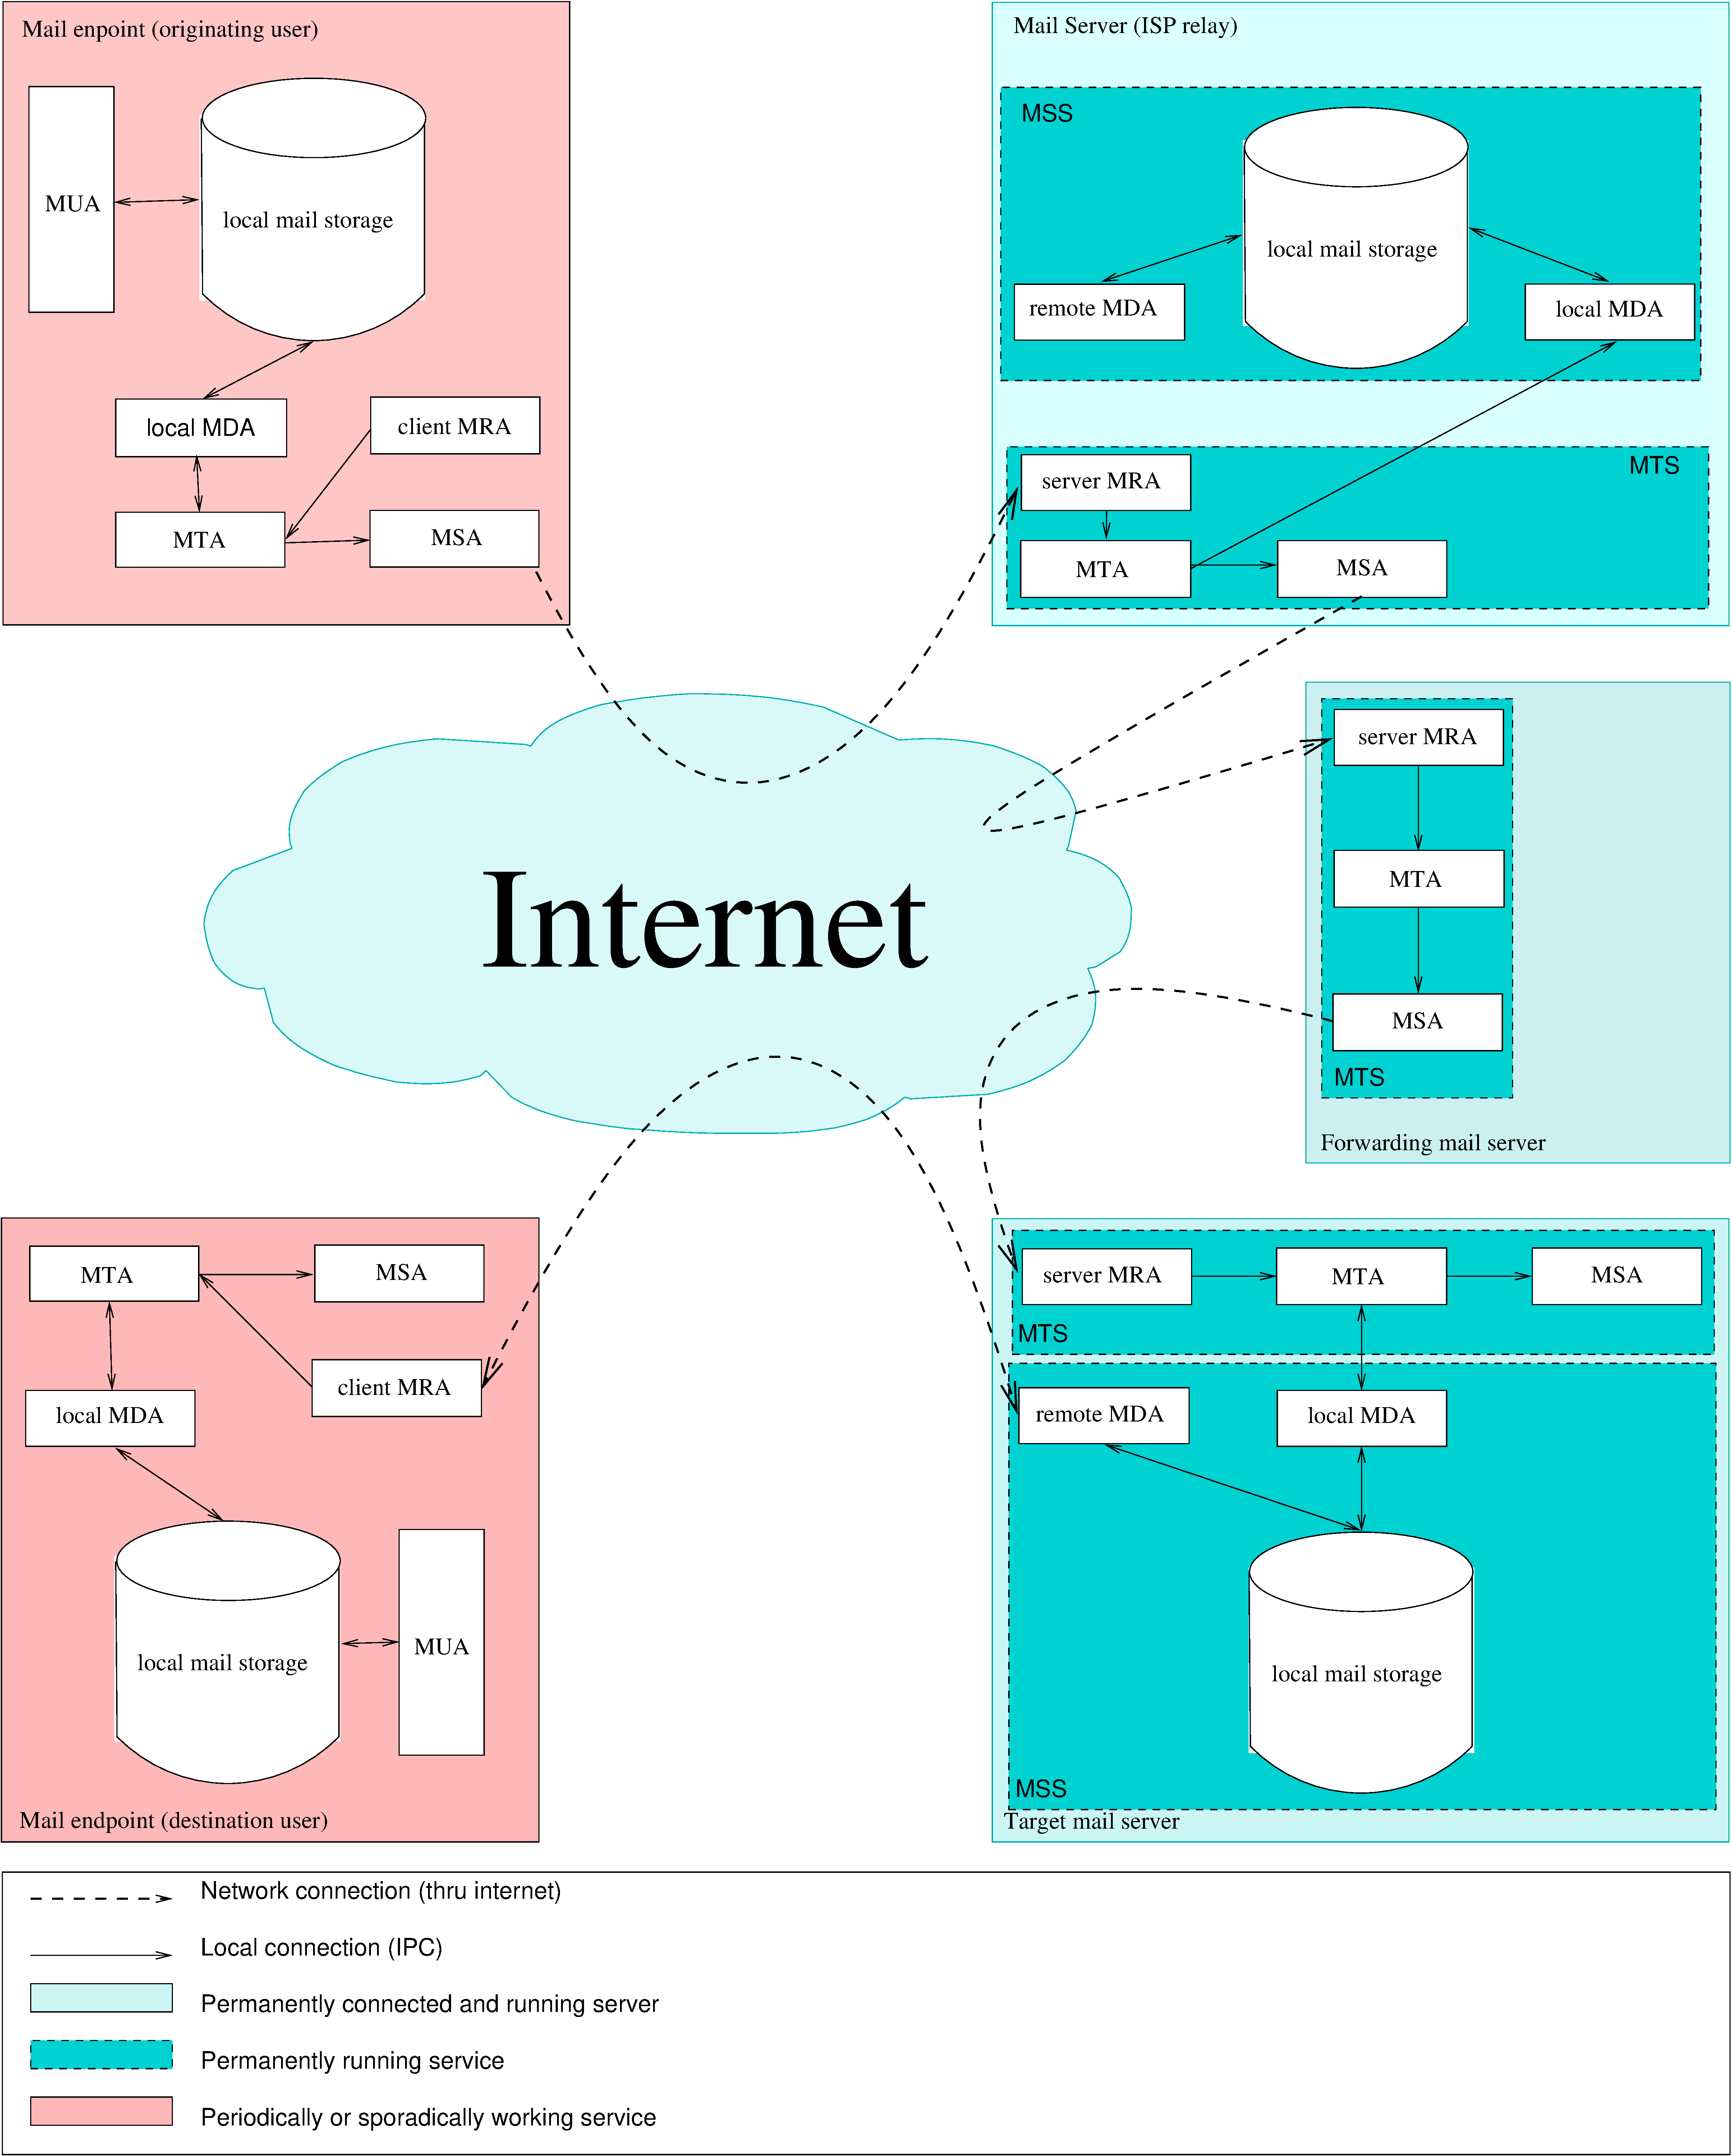
\includegraphics[width=\columnwidth]{inc/MailAgents1.pdf}
	\caption{Mail Agents}
	\label{fig:MailAgents}
\end{figure}

In the following paragraphs (for definitions), the term ``email'' is used synonymously to the term ``Message''.  ``Email'' has been chosen over ``messages'' because of its frequent use in standard documents.

Emails are typically initiated by a Mail User Agent (\defref{MUA}). An MUA accesses local email storage, which may be the server storage or a local copy. The local copy may be a cache only copy, the only existing storage (when emails are fetched and deleted from the server after retrieval), or a collected representation of multiple server storages (cache or authoritative).

Besides the MUA, the only other component accessing local email storage is the Mail Delivery Agent (\defref{MDA}). An MDA is responsible for storing and fetching emails from the local mail storage. Emails destined for other accounts than the current one are forwarded to the MTA. Emails destined to a User are persistently stored in the local email storage. It is essential to understand that email storage does not necessarily reflect a single mailbox. It may as well represent multiple mailboxes (e.g., a rich client-serving multiple IMAP accounts) or a combined view of multiple accounts (e.g., a rich client collecting mail from multiple \defref{POP} accounts). In the case of a rich client, the local MDA is part of the user agent's software. In the case of an email server, the local MDA is part of the local email store (not necessarily of the mail transport service).

On the server-side, there are usually two components (services) at work. A ``Mail Transport Service'' (\defref{MTS}) responsible for mail transfers, and a ``Mail Storage System'' which offers the possibility to store received Mails in a local, persistent store.\par

An MTS generally consists out of three parts. For incoming connects, there is a daemon called Mail Receiving Agent (\defref{Server MRA}) is typically a \defref{SMTP} listening daemon. A Mail Transfer Agent (\defref{MTA}) is responsible for routing, forwarding, and rewriting emails. Moreover, a Mail Sending Agent (\defref{MSA}) is accountable for transmitting emails reliably to another Server MRA (usually sent via \defref{SMTP}).\par

An MSS consists of local storage and delivery agents, which offer uniform interfaces to access the local store. They also deal with replication issues, and grant should take care of the atomicity of transactions committed to the storage. Typically there are two different kinds of \defref{MDA}s. \defref{Local MDA}s offer possibilities to access the store via efficient (non-network based) mechanisms (e.g., IPC or named sockets). This is usually done with a stripped-down protocol (e.g., \defref{LMTP}). For remote agents, there a publicly -- network-based -- agent available. Common Protocols for this \defref{Remote MDA}\ include \defref{POP}, \defref{IMAP}, or \defref{MS-OXCMAPIHTTP}.\par

Mail endpoints consist typically of the following components:
\begin{itemize}
	\item A Mail User agent (\defref{MUA})
	\item A Local Mail storage (\defref{MUA})
	\item A Local Mail Delivery Agent (\defref{Local MDA})
	\item A Mail Transfer Agent (\defref{MTA})
	\item A Mail Sending Agent (\defref{MSA})
	\item A Mail Receiving Agent (\defref{MRA})
\end{itemize}

Only two of these components do have external interfaces. These are \defref{MSA} and \defref{MRA}. \defref{MSA} usually uses \defref{SMTP} as transport protocol. When doing so, there are a couple of specialties. 
\begin{itemize}
	\item Port number is 587 (specified in \cite{rfc4409}).\\
	Although port numbers 25 and 465 are valid and usually have the same capabilities, they are only for mail routing between servers. Mail endpoints should no longer use them.
	\item Connections are authenticated.\\
	Unlike normal server-to-server (relay or final delivery) SMTP connections on port 25, the server should always authenticate clients of some sort. This may be based on data provided by the user (e.g., username/password or certificate) or data identifying the sending system (e.g., IP address)\cite{rfc4409}. Failure in doing authentication may result in this port being misused as a sender for \defref{UBM}.
\end{itemize}

Mail User Agents (MUA) are the terminal endpoint of email delivery. Mail user agents may be implemented as fat clients on a desktop or mobile system or as an interface over a different generic protocol such as HTTP (Web Clients). 

Server located clients are a special breed of fat clients. These clients share the properties of fat clients except that they do not connect to the server. The client application itself has to be run on the server where the mail storage persists. This makes delivery and communication with the server different. Instead of interfacing with an MSA and a client MDA, they may directly access the server's local mail storage. The local mail storage may be implemented as a database in a user-specific directory structure on these systems.

\subsubsection*{Fat clients}
The majority of mail clients are fat clients. These clients score over the more centralistic organized web clients in the way that they may offer mail availability even if an Internet connection is not available (through client-specific local mail storage). They furthermore provide the possibility to collect emails from multiple sources and store them in the local storage. Unlike Mail servers, clients are assumed to be not always online. They may be offline most of the time. To guarantee the availability of a particular email address, a responsible mail server for a specific address collects all emails (the \defref{MSS} does this). It provides a consolidated view of the database when a client connects through a local or remote MDA.

As these clients vary heavily, it is mandatory for the MDA that they are well specified. Lack of doing so would result in massive interoperability problems. Most commonly the Protocols \defref{IMAP}, \defref{POP} and \defref{EWS} are being used these days. For email delivery, the SMTP protocol is used. 

Fat clients are commonly used on mobile devices. According to  \cite{clientDistribution} in Aug 2012, the most typical fat email client was Apple Mail client on iOS devices ($35.6\%$), followed by Outlook ($20.14\%$), and Apple Mail ($11\%$). \citetitle{clientDistribution2}\cite{clientDistribution2} as a more recent source lists in February 2014 iOS devices with $37\%$, followed by Outlook ($13\%$), and  Google Android ($9\%$).

\subsubsection*{Server located clients}
Server located clients build an absolute minority. This kind of client was common in the days of centralized hosts. An example for a Server Located Client is the Unix command ``mail''. This client reads email storage from a file in the user's home directory.

\subsubsection*{Web clients}
Web clients are these days a common alternative to fat clients. Most big provider companies use their proprietary web client. According to \cite{clientDistribution2} the most common web clients are "`Gmail"', "`Outlook.com"', and "`Yahoo! Mail"'. All these Interfaces do not offer a kind of public plug-in interface. However,  they do offer IMAP-interfaces. This important for a future generalistic approach to the problem.

\section*{S/MIME (1996)}
S/MIME is an extension of the MIME standard. The MIME standard allows in simple text-oriented mails an alternate representation of the same content (e.g., as text and as HTML) or splitting a message into multiple parts that may be encoded. It is important to note that MIME encoding is only effective in the body part of a mail.

S/MIME, as described in \cite{rfc3851}, S/MIME extends this standard with the possibility to encrypt mail content or sign it. Practically this is achieved by either putting the encrypted part of the signature into an attachment. It is essential to know that this method leaks significant pieces of the data.

As the mail travels directly from sender to recipient, both involved parties are revealed. Neither message subject nor message size or frequency is hidden. This method does offer limited protection when assuming an adversary with interest in the message content only. It does not protect from the kind of adversary in our case. 

The trust model is based on a centralistic approach involving generally trusted root certification authorities.

\section*{Pretty Good Privacy (1996)}
Exactly as S/MIME, PGP\cite{rfc4880} builds upon the base of MIME. Since the trust model in PGP is peer-based, the encryption technology does not significantly differ (as seen from the security model).

Like S/MIME, PGP does not offer anonymity. Sender and endpoints are known to all routing nodes. Depending on the version of PGP, some meta-information or parts of the message content such as subject line, the sender and receiver's real name, and message size are leaked.

A good thing to learn from PGP is that peer-based approaches are offering limited possibilities for trust. The trust in PGP is based on the peer review of users. This peer review may give an idea of how well verified the key of a user is.

\section*{XMPP}
XMPP (or formerly Jabber) is defined in the RFCs \cite{rfc6120,rfc6121,rfc3923,rfc3922} and features an own extension process on the base of XEPs. The community is very active in the development and has almost 200 proposed, draft, active, final, or experimental XEPs. 

At its core, XMPP is an open, secure, decentralized, and extensible standard for real-time capable protocol, allowing to transfer messages and signal status data efficiently. It allows single or multi-user chat and may be used as dialing protocol voice, video file transfer, and similar content.

We use XMPP in our work as proof of concept that a switch of protocols (in our case, SMTP and XMPP) is doable.

The fact that the two protocols differ in their cores significantly makes it an ideal use-case. XMPP is synchronous (whereas SMTP is asynchronous, is not MIME-based (whereas SMTP is)), and has an own implementation for file transfers. On the other hand, it offers many advantages, such as the availability of end-to-end encryption or additional store-and-forward services.


\chapter[Information in Anonymizing Protocols]{Information Routing and Distribution for Anonymizing Protocols}
Information routing and distribution is not a novelty in privacy research. Researchers around the globe have searched for means of privacy.  One good example was the patent in the intro of Almon B. Strowger\cite{pulseDialingPatent}. More recent activities are the infamous "How to share a secret"\cite{shamir1979share}, which used Lagrange polynomials to distribute shares of information across multiple hosts for privacy. A single polynomial would be attackable. Shamir applied a $\mod p$ operation to hide characteristics of a curve (as long as $p$ is large and prime). The system had many problems which were addressed by subsequent work such as \cite{tompa1989share}.

Lagrange polynomes form an essential part when it comes to networking and privacy. They are commonly used in the form of Reed-Solomon codes for securing unreliable connections (e.g., \cite{aiache2008reed}), distributing data \cite{shamir1979share}.

Our approach will be to use Lagrange not primarily for distributing data but to generate unidentifiable decoy traffic. When applying a Lagrange polynomial to a message, all factors contain parts of the original message. Given enough factors of the polynomial, anyone may reconstruct the original message. As a result, an adversary cannot tell which parts of the traffic are decoy and which part is message as all parts can recover the original message.

\section{Mixing\label{sec:mixNets}}
Mixes have been first introduced by \citetitle{CHAUM1}\cite{CHAUM1} in \citeyear{CHAUM1}. The basic concept in a mix goes as follows. We do not send a message directly from the source to the target. Instead, we use a proxy server or router in between, which picks up the packet, anonymizes it, and forwards it to the recipient or another mix. If we assume that we have at least three mixes cascaded, we then can conclude that:
\begin{itemize}
	\item Only the first mix knows the true sender
	\item All intermediate mixes know neither the true sender nor the true recipient (as the data comes from mixes and is forwarded to other mixes) 
	\item Only the final mix knows the final recipient.
\end{itemize}

This approach (in this simple form) has several downsides and weaknesses.

\begin{itemize}
	\item In a low latency network, an adversary may trace the message by analyzing the timing of a message.
	\item We can emphasize a path by replaying the same message multiple times (assuming we control an evil node), thus discovering at least the final recipient.
	\item If we can ``tag'' a message (with content or attribute), we may follow the message.
\end{itemize}

In \citeyear{RP03-1} \citeauthor{RP03-1} analyzed the suitability for mixes as an anonymizing network for masses. They concluded that there are three possibilities to run mixes.
\begin{itemize}
	\item Commercial, static MixNetworks
	\item Static MixNetworks operated by volunteers
	\item Dynamic MixNetworks
\end{itemize}
They concluded that in an ideal implementation, a dynamic mix network where every user is operating a mix is the most promising solution as static mixes always might be hunted by an adversary.

\section{Anonymous Remailers\label{sec:remailers}}
Remailers have been in use for quite some time. There are several classes of remailers, and all of them are somehow related to Mixnets. There are ``types'' of remailers defined. Although these ``types'' offer some hierarchy, none of the more advanced ``types'' seem to have more than one implementation in the wild. 

Pseudonymous Remailers (also called Nym Servers) take a message and replace all information pointing to the original sender with a pseudonym. This pseudonym may be used as an answer address. The most well known pseudonymous remailer possibly was anon.penet.fi run by Johan Helsingius. Several times, this service has been forced to reveal a pseudonym's true identity before Johan Heösingius decided to shut it down. For a more in-depth discussion of Pseudonymous Remailers, see \ref{sec:remPseudo}

Cypherpunk remailers forward messages like pseudonymous remailers. Unlike pseudonymous remailers, Cypherpunk remailers decrypt a received message, and its content is forwarded without adding a pseudonym. A reply to such a message is not possible. They may, therefore, be regarded as an ``decrypting reflector'' or a ``decrypting mix'' and may be used to build an onion routing network for messages. For a more in-depth discussion of type-1-remailers, see section  \ref{sec:remCypherpunk}.

Mixmaster remailers are very similar to Cypherpunk remailers. Unlike them, Mixmaster remailers hide the messages, not in an own protocol, but use \defref{SMTP} instead. While using \defref{SMTP} as a transport layer, Cypherpunk remailers are custom (non-traditional mail) servers listening on port 25. For a more in-depth discussion of type-2-remailers, see section \ref{sec:remMixmaster}.

Mixminion remailers extend the model of Mixmaster remailers. They still use \defref{SMTP} but introduce new concepts. New concepts in Mixminion remailers are:
\begin{itemize}
	\item Single Use Reply Blocks (SURBs)
	\item Replay prevention
	\item Key rotation
	\item Exit poicies
	\item Dummy traffic
\end{itemize}
For a more in depth discussion of Mixminion remailers see section \ref{sec:remMixminion}.


\section{Onion Routing}
Onion routing is a further development of the concept of mixes. In onion routers, every mix gets a message which is asymmetrically encrypted. By decrypting the message, he obtains the next-hops name and the content he has to forward. The main difference in this approach is that the mix decides about the next hop in traditional mix cascades. In an onionised routing system, the message chooses the route it is taking. 

Onionized messages typically have the problem of a constant size loss throughout the system. Some systems counter this effect, y separating the routing setup from the message path.

While tagging attacks are far more demanding (if we exclude side-channel attacks to break sender anonymity), the traditional attacks on mixes are still possible. So when an adversary is operating entry and exit nodes, it is straightforward for them to match the respective traffic.

One very well known onion routing network is Tor (\href{https://www.torproject.org}{https://www.torproject.org}). For more information about Tor see section \ref{sec:tor}.

\section{Garlic Routing}
Garlic routing is an improved form of onion routing. To stop onionized messages from continuously loose contents through their way, a garlic router collects multiple, independent messages into one message before routing. This compensates for the ``size loss effect'' of onionized systems.

\section{Crowds}
Crowds is a network that offers anonymity within a local group. It works as follows:

\begin{itemize}
	\item All users add themselves to a group by registering on a so-called ``blender''.
	\item All users start a service (called JonDo).
	\item Every JonDo takes any received message (might be from him as well) and sends it with a 50\% chance either to the correct recipient or to a randomly chosen destination
\end{itemize}

While crowds, as specified in \cite{crowds:tissec}, does anonymize the sender from the recipient rather well, the system offers no protection from someone capable of monitoring crowds traffic. The system may, however, be easily attacked from within by introducing collaborating jondos. It has been further developed to D-Crowds \cite{crowdsAttack}, ADU/RADU \cite{Munoz-Gea2008}, Freenet\cite{freenet} and others. 

Furthermore, the blender is aware of all JonDos and thus of particular interest for any observing or censoring adversary. Control of the blender enables an adversary to split the network into controllable parts, adding a high likelihood of discovering an original sender.

\section{Mimic Routes}
Mimics are a set of statical mixes that maintain a constant message flow between the static routes. If legitimate traffic arrives, the pseudo traffic is replaced by legitimate traffic. An outstanding observer is thus incapable of telling the difference between real traffic and dummy traffic.

If centralized mixes are used, the system lacks the same vulnerabilities of sizing and observing the exit nodes as all previously mentioned systems. If we assume that the sender and receiver operate a mixer by themselves, the system would no longer be susceptible to timing or sizing analyses. The mimic routes put a constant load onto the network. This bandwidth is lost and may not be reclaimed. It does not scale well as every new participant increases the need for mimic routes and creates (in the case of user mixes) a new mimic load. Furthermore, the mixes are easily identifiable as their characteristic data stream contrasts with other network service streams.

\section{Distributed Hash Tables}
Anonymous file transfer is quite often based on Distributed Hash Tables (DHTs). Systems like $I^2P$, Freenet, or Classified-ads base on DHT.

In most anonymity systems using DHT, DHTs are either used to cloak the hashed nodes while enabling routing to them or to build complex anycast structures.
%\fxwarning{complete section}

\section{Dining Cryptographer Networks}
DC networks are based on the work \citetitle{chaum-dc} by \citeauthor{chaum-dc}\cite{chaum-dc}. In this work, \citeauthor{chaum-dc} describes a system allowing a one-bit transfer (The specific paper talks about the payment of a meal). Although all the DC net participants are known, the system makes it unable to determine who has been sending a message. The message in a DC-Net is readable for anyone. This network has the downside that a cheating player may disrupt communication without being traceable.

Several attempts have been made to strengthen the proposal of Chaum\cite{golle:eurocrypt2004,disco,herbivore:tr,Corrigan-Gibbs:2010:DAA:1866307.1866346}. However, no one succeeded without introducing significant downsides on the privacy side.

\section{Private Information Retrieval}
Private Information Retrieval (PIR)\cite{chor1995private} was developed by \citeauthor{chor1995private}. It is a  public database organized in Slots where some clients write into specific slots and other clients access the whole database so that the server is unable to tell what data was accessed. It is a simplified or weaker version of an oblivious transfer (1-out-of-n). PIR was described in theory and had two different approaches. A computationally secured approach (cPIR), which is the weaker of two approaches, and the information-theoretic secured approach (itPIR).

PIR was the foundation or an inspiration for many other systems and extensions such as CSPIR\cite{lipmaa2009first}, BddCpir\cite{lipmaa2009first}, Popcorn\cite{gupta2016scalable}, or Riposte\cite{corrigan2015riposte}.

\chapter[Academic Protocols and Implementations]{Proposed Academic Protocols and Implementations}\label{sec:implSystems}
In this section, we list various proposed anonymity systems regardless of their age or state. We analyze their inner working and try to compare them in a unified way. This comparison was a base for selecting our approach.


\section{Characteristics of Known Anonymity Implementations}
Table \ref{tab:anonClass} shows the protocols analyzed in the next sections ordered by type and year according to the classification scheme introduced in \cite{Shirazi2018}.

\gdef\cc{}
\gdef\cols{
	\ifx\cc\empty
		\gdef\cc{not empty}
	\else
		\gdef\cc{}
	\fi
	\col
}
\gdef\col{%
\ifx\cc\empty%
\cellcolor{black!30}%
\else%
\cellcolor{black!10}%
\fi}
	
\gdef\mybull{\medbullet}
\gdef\mycirc{\medcirc}
\gdef\mytick{\faCheck}
\gdef\mycross{\faTimes}
% network
%\usepackage{ amssymb }
\newcommand\networkFully{$\col\boxtimes$}
\newcommand\networkMostly{\col$\square$}
\newcommand\networkPartly{\col$\sqsubset$}
%direction
\newcommand\directionBidi{\col$\longleftrightarrow$}
\newcommand\directionUnidi{\col$\longrightarrow$}
% synchronization
\newcommand\syncAsync{\col$\neq$}
\newcommand\syncSynchronous{\col$\cong$}
% symmetry
\newcommand\rolePtp{\col\scalebox{0.4}{$\mybull\cdot\cdot\mybull\cdot\cdot\mybull$}}
\newcommand\roleCs{\col\scalebox{0.4}{$\mybull\cdot\cdot\mybull$}}
\newcommand\roleHybrid{\col\scalebox{0.4}{$\mybull\cdot\cdot\mycirc\cdot\cdot\mybull$}}
% Hierarchy
\newcommand\hierarchyFlat{\col$\cdots$}
\newcommand\hierarchyHierarchical{\col\ding{68}}
% centralization
\newcommand\decentralizationPart{\col\astrosun}
\newcommand\decentralizationDecentr{\col$\bigcirc$}
\newcommand\decentralizationNo{\col\mycross}
% Network view
\newcommand\netviewFully{\col$\CIRCLE$}
\newcommand\netviewPartly{\col$\LEFTcircle$}
% NW updating
\newcommand\updatingTimed{\col\clock}
\newcommand\updatingEvent{\col\lightning}
\newcommand\updatingNoupd{\col\mycross}
% Routing
\newcommand\routingRoutesrc{\col\scalebox{0.4}{$\mybull\cdots$}}
\newcommand\routingRoutehop{\col\scalebox{0.4}{$\cdots\mybull\cdots$}}
\newcommand\routingRoutebc{\col\faBullhorn}
% Sheduling
\newcommand\shedfair{\col$\equiv$}
\newcommand\shedprio{\col$\Diamonddot$}
%determinism
\newcommand\nsdetdet{\col\mytick}
\newcommand\nsdetprob{\col\mycross}
%selection set
\newcommand\nsnodesall{\col\CircledA}
\newcommand\nsnodessec{\col\Stopsign}
\newcommand\nsnodesnet{\col\Mundus}
\newcommand\nsnodesusr{\col\smiley}
% probability
\newcommand\nsprobuni{\col$\circledast$}
\newcommand\nsprobstat{\col$\circledcirc$}
\newcommand\nsprobdyn{\col$\ast$}
% latency
\newcommand\perflatl{\col L}
\newcommand\perflath{\col H}
\newcommand\perflatm{\col M}
% mode 
\newcommand\perfmodecon{\col$\multimapdotboth$}
\newcommand\perfmodemsg{\col\Letter}
% implementation
\newcommand\nsimplyes{\col\mytick}
\newcommand\nsimplno{\col\mycross}
% code available
\newcommand\nscodeyes{\col\mytick}
\newcommand\nscodeno{\col\mycross}
% context
\newcommand\nscontmsg{\faEnvelope}
\newcommand\nscontmail{@}
\newcommand\nscontbulletin{\faUsers}
\newcommand\nscontphone{\Telefon}
\newcommand\nscontwww{\faInternetExplorer}
\newcommand\nscontmicroblog\faPencil
\newcommand\nscontfiles\faStickyNote
\newcommand\nscontwifi\faWifi
\newcommand\nscontBC{\faBullhorn}

\DeclareFixedFootnote{\takenFrom}{Definition taken from \cite{Shirazi2018}}
\begin{table*}[ht]\centering\tiny
	\setlength{\aboverulesep}{0pt}
	\setlength{\belowrulesep}{0pt}
	\newcolumntype{x}[1]{!{\centering\arraybackslash\vrule width #1}}
	\gdef\swidth{0.18cm}
	\gdef\wwidth{0.36cm}
	%\rowcolors{8}{black!30}{black!10}
	\begin{tabular}{x{2pt}clx{2pt}*{5}{p{\swidth}|}p{\swidth}x{2pt}p{\swidth}|p{\swidth}x{2pt}*{4}{p{\swidth}|}p{\swidth}x{2pt}*{4}{p{\swidth}|}p{\wwidth}x{2pt}}
		\toprule
		
		& & \multicolumn{6}{cx{2pt}}{Network structure} & \multicolumn{2}{p{\wwidth}x{2pt}}{\centering Routing \\ info} & \multicolumn{5}{cx{2pt}}{Communication model} & \multicolumn{5}{cx{2pt}}{Performance and deployability}\\\cmidrule{3-20}
		
		& & & \multicolumn{2}{c|}{Connect} & \multicolumn{3}{cx{2pt}}{Symmetry} & & & & & \multicolumn{3}{cx{2pt}}{Node selection} & & & & & \\\cmidrule{4-5}\cmidrule{6-8}\cmidrule{13-15}
		
		& & \rot{Topology} & \rot{Direction} & \rot{Synchronization} & \rot{Roles} & \rot{Hierarchy} & \rot{Decentralization} & \rot{Network view} & \rot{Updating} & \rot{Routing Type} & \rot{Scheduling} & \rot{Determinism} & \rot{Selection set} & \rot{selection probability} & \rot{Latency} & \rot{Communication mode} & \rot{Implementation} & \rot{Code availability} & \cellcolor{white}\rot{Context/application} \\
		\midrule
	
		\parbox[t]{6pt}{\multirow{14}{*}{\rot{\parbox[c]{4.2cm}{\centering Resenders, onion routers and mixes}}}} &  \cols Chaum Mixes\takenFrom & \networkFully & \directionUnidi & \syncAsync & \roleCs & \hierarchyFlat & \decentralizationNo & \netviewFully & \updatingNoupd & \routingRoutesrc & \shedfair & \nsdetdet &  \nsnodesall & \nsprobstat & \perflath & \perfmodemsg & \nsimplyes & \nscodeno & \col\nscontmail \\
		
		& \cols Babel\takenFrom & \networkFully & \directionUnidi & \syncAsync & \roleCs & \hierarchyFlat & \decentralizationPart & \netviewFully & \updatingNoupd & \col\centering\begin{minipage}{\swidth}\routingRoutesrc \\ \routingRoutehop\end{minipage} & \shedfair & \nsdetdet &  \nsnodesall & \nsprobuni & \perflath & \perfmodemsg & \nsimplno & \nscodeno & \col\nscontmail \\
		
		&\cols Mixmaster\takenFrom & \networkFully & \directionUnidi & \syncAsync & \roleCs & \hierarchyFlat & \decentralizationPart & \netviewPartly & \updatingNoupd & \routingRoutesrc & \shedfair & \nsdetprob &  \nsnodesall & \nsprobuni & \perflath & \perfmodemsg & \nsimplyes & \nscodeyes & \col\nscontmail \\
		
		&\cols Crowds\takenFrom & \networkFully & \directionBidi & \syncAsync & \rolePtp & \hierarchyFlat & \decentralizationPart & \netviewFully & \updatingEvent & \routingRoutehop & \shedfair & \nsdetprob &  \nsnodesall & \nsprobuni & \perflatl & \perfmodemsg & \nsimplyes &\nscodeno & \col\nscontwww \\
		
		&\cols Tor\takenFrom & \networkPartly & \directionBidi & \syncSynchronous & \roleHybrid & \hierarchyFlat & \decentralizationPart & \netviewFully & \updatingTimed & \routingRoutesrc & \shedfair & \nsdetprob &  \nsnodesnet \nsnodessec & \nsprobstat & \perflatl & \perfmodemsg & \nsimplyes & \nscodeyes & \col\nscontwww \\
		
		&\cols $I^2P$\takenFrom & \networkMostly & \directionUnidi  & \syncAsync & \rolePtp & \hierarchyFlat & \decentralizationDecentr & \netviewFully & \updatingTimed & \routingRoutesrc & \shedprio & \nsdetprob & \nsnodesnet \nsnodessec & \nsprobdyn & \perflatl & \perfmodecon & \nsimplyes & \nscodeyes & \col\begin{tabular}{@{}c@{}} \nscontwww \nscontmail \\ \nscontfiles\end{tabular} \\
		
		&\cols Mixminion\takenFrom & \networkFully & \directionUnidi & \syncAsync & \roleCs & \hierarchyFlat & \decentralizationPart & \netviewFully & \updatingTimed & \routingRoutesrc & \shedfair & \nsdetprob &  \nsnodesall & \nsprobuni & \perflath & \perfmodemsg & \nsimplyes & \nscodeyes & \col\nscontmail \\
		
		&\cols $\mathcal{P}^5$\takenFrom & \networkPartly & \directionUnidi  & \syncAsync & \rolePtp & \hierarchyHierarchical & \decentralizationPart & \netviewPartly & \updatingEvent & \routingRoutebc & \shedprio & \nsdetdet & \nsnodesusr & \nsprobstat & \perflath & \perfmodemsg & \nsimplyes & \nscodeno & \col\nscontmsg\\
		
		% AN.ON missing
		
		&\cols AP3\takenFrom & \networkPartly & \directionBidi & \syncAsync & \rolePtp & \hierarchyFlat & \decentralizationDecentr & \netviewPartly & \updatingEvent & \routingRoutehop & \shedfair & \nsdetprob &  \nsnodesall  & \nsprobuni & \perflatl & \perfmodecon & \nsimplno & \nscodeno  & \col\begin{tabular}{@{}c@{}}\nscontwww\nscontmail \\ \nscontBC \end{tabular}\\
		
		% Cashmere missing
		
		&\cols SOR & \networkFully & \directionBidi & \syncSynchronous & \roleCs & \hierarchyFlat & \decentralizationDecentr & \netviewFully & \updatingNoupd & \routingRoutesrc & \shedfair & \nsdetdet & \nsnodesusr & \nsprobuni &  \perflatl & \perfmodecon & \nsimplyes & \nscodeyes & \col\nscontwww\nscontmail \\
		
		
		&\cols Vuvuzela & \networkFully & \directionBidi & \syncSynchronous & \roleCs & \hierarchyHierarchical & \decentralizationNo & \netviewFully & \updatingNoupd & \routingRoutesrc & \shedfair & \nsdetdet & \nsnodesusr & \nsprobuni &  \perflatm & \perfmodemsg & \nsimplyes & \nscodeyes & \col\nscontmicroblog \\
		
		&\cols Riffle & \networkFully & \directionBidi & \syncSynchronous & \roleHybrid & \hierarchyHierarchical & \decentralizationNo & \netviewFully & \updatingNoupd & \routingRoutehop & \shedfair & \nsdetdet & \nsnodesnet \nsnodessec & \nsprobstat & \perflatl & \perfmodemsg & \nsimplyes & \nscodeyes & \col\nscontwww \\
		
		% MCMix missing
		
		% SCION missing
		
		&\cols Karaoke & \networkFully & \directionUnidi & \syncSynchronous & \roleCs & \hierarchyHierarchical & \decentralizationNo & \netviewFully& \updatingNoupd& \routingRoutesrc& \shedfair & \nsdetprob & \nsnodesusr & \nsprobuni & \perflatl & \perfmodemsg & \nsimplyes & \nscodeno & \col\nscontBC\nscontmicroblog \\
		
		& \cols \MessageVortex & \networkFully & \directionBidi & \syncSynchronous & \rolePtp & \hierarchyFlat & \decentralizationDecentr & \netviewPartly &  \updatingEvent &  \routingRoutesrc & \shedfair & \nsdetprob & \nsnodesusr & \nsprobuni & \perflath & \perfmodemsg & \nsimplyes & \nscodeyes & \col\nscontmail \\ \hline
		
		\parbox[t]{5pt}{\multirow{2}{*}{\rot{PIR~~}}} & \cols Riposte & \networkFully & \directionUnidi & \syncSynchronous & \roleCs & \hierarchyFlat & \decentralizationPart & \netviewFully & \updatingNoupd & \routingRoutebc & \shedfair & \nsdetprob & \nsnodesall &\nsprobuni & \perflath & \perfmodemsg & \nsimplyes & \nscodeyes & \col\nscontBC\nscontmicroblog \\
		
		& \cols Pung & \networkFully & \directionBidi & \syncAsync & \roleCs & \hierarchyFlat & \decentralizationNo & \netviewFully & \updatingNoupd & \routingRoutebc & \shedfair & \nsdetdet & \nsnodesall & \nsprobuni & \perflatm & \perfmodemsg & \nsimplyes & \nscodeno & \col\nscontBC\nscontmicroblog \\\hline
		
		\parbox[t]{5pt}{\multirow{3}{*}{\rot{DHT~~~}}}& \cols Tarzan\takenFrom & \networkMostly & \directionBidi & \syncAsync & \rolePtp & \hierarchyFlat & \decentralizationDecentr & \netviewFully & \updatingEvent & \routingRoutesrc & \shedfair & \nsdetprob &  \nsnodessec  & \nsprobuni & \perflatl & \perfmodecon & \nsimplyes & \nscodeyes  & \col\nscontwww \\
		
		& \cols MorphMix\takenFrom & \networkPartly & \directionBidi & \syncAsync & \rolePtp & \hierarchyFlat & \decentralizationPart & \netviewPartly & \updatingEvent & \routingRoutehop & \shedfair & \nsdetprob &  \nsnodesnet & \nsprobdyn & \perflatl & \perfmodecon & \nsimplyes & \nscodeyes  & \col\nscontwww \\
		
		& \cols Salsa\takenFrom & \networkPartly & \directionBidi & \syncAsync & \col\centering\begin{minipage}{\swidth}\rolePtp \\ \roleHybrid \end{minipage} & \hierarchyFlat & \decentralizationDecentr & \netviewPartly & \updatingEvent & \routingRoutehop & \shedfair & \nsdetprob &  \nsnodesall  & \nsprobuni & \perflatl & \perfmodecon & \nsimplyes & \nscodeno & \col\nscontwww \\\hline
		
		\parbox[t]{5pt}{\multirow{4}{*}{\rot{DC~~}}}& \cols Chaum\'{}s DCnet\takenFrom & \networkFully & \directionUnidi  & \syncAsync & \rolePtp & \hierarchyFlat & \decentralizationNo & \netviewFully & \updatingEvent & \routingRoutebc & \shedfair & \nsdetdet & \nsnodesall & \nsprobstat & \perflath & \perfmodemsg & \nsimplno & \nscodeno & \col\nscontmsg \\
		
		& \cols Herbivore\takenFrom & \networkPartly & \directionUnidi  & \syncAsync & \rolePtp & \hierarchyHierarchical & \decentralizationPart & \netviewPartly & \updatingEvent & \routingRoutebc & \shedfair & \nsdetdet & \nsnodesnet & \nsprobstat & \perflatm & \perfmodemsg & \nsimplyes & \nscodeno & \col\nscontmsg \\
		
		& \cols Dissent in numbers\takenFrom & \networkPartly & \directionUnidi  & \syncAsync & \roleCs & \hierarchyHierarchical & \decentralizationPart & \netviewPartly & \updatingEvent & \routingRoutebc & \shedfair & \nsdetdet & \nsnodesnet & \nsprobstat & \perflath & \perfmodemsg & \nsimplyes & \nscodeyes & \col\nscontmsg \\
		
		& \cols Verdict & \networkFully & \directionUnidi & \syncSynchronous & \roleCs & \hierarchyHierarchical & \decentralizationPart & \netviewPartly & \updatingEvent & \routingRoutebc & \shedfair & \nsdetdet & \nsnodesnet & \nsprobstat & \perflath & \perfmodemsg &\nsimplyes & \nscodeyes & \col\nscontmsg \\\hline
		
		\parbox[t]{5pt}{\multirow{2}{*}{\rot{BC~}}}& \cols Hordes & \networkFully & \directionBidi & \syncAsync & \rolePtp & \hierarchyFlat & \decentralizationPart & \netviewFully & \updatingEvent & \routingRoutebc & \shedfair & \nsdetprob &  \nsnodesall & \nsprobuni & \perflatl & \perfmodemsg & \nsimplyes &\nscodeno & \col\nscontwww \\
		
		& \cols Atom & \networkPartly & \directionUnidi & \syncSynchronous & \roleCs & \hierarchyFlat & \decentralizationPart & \netviewFully & \col ? & \routingRoutesrc & \shedfair & \nsdetprob &  \nsnodesall & \nsprobuni & \perflath & \perfmodemsg & \nsimplyes & \nscodeyes & \col\nscontBC\nscontmicroblog \\\hline
		
		% Loopix & & & & & & & & & & & & & & & & & & \\
		% Stadium & & & & & & & & & & & & & & & & & & \\
		
		% Alpenhorn & & & & & & & & & & & & & & & & & & \\
		
		% Torsk\takenFrom & \networkPartly & \directionBidi & \syncAsync & \roleHybrid & \hierarchyFlat & \decentralizationPart & \netviewPartly & \updatingEvent & \routingRoutesrc & \shedfair & \nsdetprob &  \nsnodesnet  & \nsprobuni & \perflatl & \perfmodecon & \nsimplyes & \nscodeno  & \nscontwww \\
		
		\bottomrule
	\end{tabular}
	\caption{Classification table for anonymization protocols}
	\label{tab:anonClass}
\end{table*}

In the table, some historical systems have been omitted. Additionally SCION has been ommited as not fitting anywhere into the table. It may be seen as a remixing system but too many aspects have been intermixed with the routing logic to give really a clear classification. Furthermore, the SOR classification is highly speculative as this system has many aspects left out, making it hard to categorize correctly. Where the paper does not give exact indication of how this part is solved we made guesses in favor of the work.

As key indicators for similar protocols, we identified the following characteristics:
\begin{itemize}
	\item It needs to be peer-to-peer (\rolePtp) or hybrid (\roleHybrid)\\
	The hybrid role is only allowed when no dedicated servers for the protocol are required. Dedicated servers would have the downside of repression against administrators.
	\item It needs to be fully decentralized (\decentralizationDecentr)\\
	An adversary may use central infrastructures to disrupt and control infrastructures.
	\item Routing has to be source controlled (\routingRoutesrc) or broadcast-based (\routingRoutebc)\\
	In any infrastructure where mixes decide about the route, an adversary may redirect a message to nodes under his control.
	\item The nodes must be user-defined (\nsnodesusr) or the system must have information-theoretic promises that even if all nodes collaborate, the system is not compromized\\
	In every system where the security relies on nodes' trust, a user should always be in full control.
	\item The system must work in a high latency mode (\perflath)\\
	Every low/medium latency system makes promises regarding the traffic, which makes the system detectable.
\end{itemize}

Unfortunately, all of the protocols found implement their ``own'' protocol, rendering them easily censorable. 

\section{Resenders, Onion Routers, and MixNets Based Systems}\label{sec:remailersAndMixnets}
\subsection{Pseudonymous Remailers (1981)\label{sec:remPseudo}}
A pseudonymous remailer allows reaching people via a pseudonymous email address. The remailing server removes all traces of the original sender and inserts a pseudonymous email instead. The foundation of these remailers can be found in an early article by David Chaum\cite{CHAUM1}.

One of the most famous remailers was the Penet remailer (anon.penet.fi). This remailer only lasted from 1993 to 1996 and was shut down after two compromises involving the Chruch of Scientology. Details of the closure can be found in \cite{penetClosure}.

It drastically shows the problem of legal prosecution even within so-called ``democratic environments''.

\subsection{Cypherpunk Remailers (approx. 1993)\label{sec:remCypherpunk}}
With the failing of anon.penet.fi, it became clear that the weakest spot of a single server infrastructure the information stored on the server and the vulnerability of their owner. The new type-1-remailers score over the existing type-0-remailers by using encryption for the message.  The time of the invention of the first type-1-remailers is unclear. Setting up a type-1-remailer was typically achieved by using procmail together with a small script calling PGP binaries and then sending the resulting message to the next recipient. By combining multiple type-1-remailers, an onion-like structure of the message was achievable. 

This approach was promising, but it was still observable. An observation was possible by correlating the message sizes (e.g., strictly decreasing) and timing information. Furthermore, remailers were yet known, and authorities were able to ban infrastructure and capable of monitoring their routing activities. The standard mail logs of such servers provided valuable evidence for legal prosecution if not disabled.

\subsection{Babel (1996)}
Babel was an academic system defined in a paper by \citeauthor{babel} in \citeyear{babel}\cite{babel}. It has been developed at IBM Zurich Research Laboratory. It was a mixing system using onionized addresses. The sender remains anonymous while he may provide a reply routing block called RPI. If both parties want to remain anonymous, the initiator's RPI was deployed in a forum thread. Anyone using this block adds an RPI for its address to the message.

This system has all the disadvantages of a system using MURBs. Traffic highlighting, timestamp, and similar attacks are possible. Furthermore, the source of the RPIs on the message board was by design unclear and, therefore, not trustworthy.

\subsection{Mixmaster-Remailers (1996)\label{sec:remMixmaster}}
Like Cypherpunk remailers, the Mixmaster remailers were working with onion-like encrypted messages. The protocol was based on Chaum's Mix-Nets in \cite{CHAUM1} and further developed by L. Cotrell in 1996. 

In contrast to type-1-remailers, the use of cascading systems to remail became systematic. The end-user used specialized software to build and send Mixmaster messages.

Mixmaster messages were still traceable by message size. The system did not support reply blocks. A user had to know all Mixmaster nodes to use the system. The last node was typically an exit node sending the message in clear to the final recipient. This behavior still allowed the use of Usenet.

\subsection{Crowds (1997)}
Crowds is an anonymity network for browsing and was the starting point for many similar systems such as D-Crowds, AN.ON and may be seen as a predecessor for Tor specialized in forwarding HTTP requests. 

In Crowds, a user joins a crowd by registering at the blender node of a Crowd network a jondo service. The network has, besides the blender, a variable number of nodes called jondos. These nodes are forwarding nodes that either send a message to another random jondo (including themselves) or forward it to the final recipient. The behavior is chosen based on a probability factor. The behavior is constant for a period (connection) and renegotiated from time to time (usually hourly). Furthermore, jondos are required to strip any personal information from a request. 

A jondo acts as a proxy for a web browser or other jondos. Therefore, jondos' have plain text access to the routed requests and replies. Messages between jondos' are symmetrically encrypted. From the senders' point, Crowds offers perfect anonymity towards the receiver. 

While the concept of blending into a crowd of members was inspiring for many other solutions, it has specific weaknesses. Jondos may be collaborating, or the blender may create subnetworks of collaborating jondos' to break anonymity. Furthermore, the strict forwarding property makes it susceptible to the predecessor attack\cite{wright2004predecessor}, which intersects multiple (past) paths striving to reduce the anonymity set down to isolate the originating node.

\subsection{Tor (2000)}\label{sec:tor}
Tor is one of the most common onion router networks these days and onionizes generic TCP streams. It is specified in \cite{tor-spec}. It might be considered one of the most advanced networks since it has a considerable size, and much research has been done here.

According to \cite{onion-routing:pet2000} Tor is a network consisting of multiple onion routers. Each client first picks an entry node. It establishes an identity, gets a listing of relay servers, and chooses a path through multiple onion routers. The temporary identity links to such a path and should be changed regularly along with its identity. Transferring data works by splitting the data into equally sized cells of 512 bytes.

There is a centrally organized directory in the Tor network, knowing all tor relay servers. Any Tor relay server may be a directory server as well. 

Many attacks involving the Tor networks have been discussed in the academic world such as \cite{hs-attack06,esorics13-cellflood,bauer:wpes2007,esorics12-torscan,oakland2013-trawling,danner-et-al:tissec12,congestion-longpaths} and some have even been exploited actively. In the best case, the people discovering the attacks did propose mitigation to the attack. Some of these mitigations flowed back into the protocol. Some general thoughts of the attacks should be emphasized here for treatment in our protocol.

Being an exit node may be a problem in some jurisdictions. In general, it seems to be accepted that routing traffic with unknown content (to the routing node) is not regarded as illegal per se. By being unable to tell malicious or illegal traffic apart from legitimate traffic, this is not a problem. However -- being an exit node can mean that unencrypted and illegal traffic is leaving the routing node. In this specific case, operators of a relay node might fear legal prosecution. Tor nodes may proclaim themselves as  ``non-exit nodes''  to avoid the possibility of legal prosecution.

Furthermore, several DoS-Attacks have been carried out to overload parts of the Tor network. Most of them do a bandwidth drain on the network layer.

Attacking anonymization has been done in several ways. First of all, the most common attack is a time-wise correlation of packets if in control of an entry and an exit node. A massive attack of this kind was published in 2014 and has been published on the Tor website (\href{https://blog.torproject.org/blog/tor-security-advisory-relay-early-traffic-confirmation-attack}{relay early traffic confirmation attack}). This attack was possible because Tor is a low latency network. Another attack is to identify routes through Tor by statistically analyze the traffic density in the network between nodes. More theoretical attacks focus on the possibility of controlling the directory servers to guarantee that an entity may be deanonymized because it is using compromised routers. A generic analysis of low latency systems also relevant for Tor can be found in \cite{johnson2009design}.

Generally, the effectiveness of the monitoring of single nodes or whole networks is disputed. According to a study by \citeauthor{ccs2013-usersrouted} in \citeyear{ccs2013-usersrouted}\cite{ccs2013-usersrouted}, a system in the scale of PRISM should be able to correlate traffic of 95\% of the users within a ``few days''. Other sources based on the Snowden Papers claim that NSA was unable so far to deanonymize users of  Tor. However, since these papers referenced ``manual analysis'', the statement may be disputed when looking at automated attacks.

According to \url{https://www.torproject.org/docs/pluggable-transports}, it is impossible to use transborder Tor traffic in at least China, Uzbekistan, Iran, and Kazakstan. In censored countries, Tor offers so-called bridged Transports. Currently deployed transports in the standard Tor browser bundle package are obfs4, meek, FTE, and ScrambleSuit. Only meek is listed as working in China. Meek achieves this by hiding its traffic in a standard protocol (https) and using public proxies such as Appspot.

\cite{saleh2018shedding} is an excellent survey listing recent developments and attacks within the Tor project.

\subsection{\texorpdfstring{$I^2P$}{I2P} (2001)}
The name $I^2P$ is a derived from  ``Invisible Internet Project'' according to \href{https://geti2p.net/}{geti2p.net}. The first binary release on SourceForge dates from 2001. The system itself is comparable to Tor for its capabilities. Mayor differences are:
\begin{itemize}
	\item P2P based
	\item Packet-switched routing (Tor is ``circuit-switched'')
	\item Different forward and backward routes (called tunnels)
	\item Works pseudonymously
	\item Supports TCP and UDP
\end{itemize}

$I^2P$ has not attracted as much attention as Tor so far. So it is hard to judge upon its real qualities.

In \citeyear{pets2011-i2p} \citeauthor{pets2011-i2p} presented in \cite{pets2011-i2p} an attack. As $I^2P$s security model is chosen based on IP addresses, the authors propose to use several cloud providers in different B-Class networks. By selectively flooding peers, an adversary may extract statistical information. The paper proposes an attack based on the heuristic performance-based peer selection. The paper's main critics were that the peer selection might be influenced by an adversary, enabling him to recover data on a statistical base.

\subsection{Mixminion-Remailers (2002)\label{sec:remMixminion}}
Mixminion was the standard implementation of a type-3-remailer. It tried to address many previously unsolved issues. 

A Mixminion router splits messages in equally sized chunks and supports SURBs. Furthermore,  replay protection and key rotation were available. Unlike the previous remailer types, Mixminion was no longer using \defref{SMTP} as the transport protocol. Instead, Mixminion introduced a new transport protocol. The sources of this remailer are available on GitHub under \url{https://github.com/mixminion/mixminion}.

As a received message had to be decoded by the final recipient. Therefore, the final recipient had to be aware of the Mixminion system.

Mixminion-Networks have been privacy-wise criticised for the following things: 
\begin{itemize}
	\item Pseudonymous single use reply blocks are broken (Chapter 4.2 in \cite{sassamanpynchon}).
	\item Central directory of mixes.
	\item Too few users
\end{itemize}

According to \url{https://mixminion.net}, the software's first release was in December 2002 and has been discontinued in 2008. Since 2011 the sources are available on GitHub. There have been forks in 2011, but currently, all forks seem to be inactive since at least 2016 as there are no new commits.

\subsection{\texorpdfstring{$\mathcal{P}^5$}{P5} (2002)}
The Peer-to-Peer Personal Privacy Protocol is defined in \cite{sherwood-protocol}. It provides sender-, receiver- and sender-receiver anonymity. According to the project page of $\mathcal{P}^5$, there is only a simulator available for the protocol.

The transport layer problem has been wholly ignored, as there is no precise protocol specification. As there is only a rough outline of the messaging and the crypto operations, $\mathcal{P}^5$ offers minimal possibilities for analysis.

\subsection{AN.ON (2003)}
AN.ON, as suggested in \cite{federrath2003system}, is a mixing network. It generates messages in equally sized chunks and sends them in fixed time slots after random mixing. Its implementation is called JAP and may be found under https://anon.inf.tu-dresden.de/. JAP is in many ways similar to the capabilities of Tor. The network was at the time of writing a lot smaller (10 JonDos compared to 6500 relays in the Tor network).

While the approach is both simple and effective, it is not suitable against a powerful adversary. First, an adversary may be able to snoop the forwarding when on the system. Second, due to the timing behavior, tunnels belonging to each other may be identified, and third, the package size information does leak as well.

\subsection{AP3 (2004)}
AP3, as defined in \cite{mislove2004ap3}, is an anonymous communication system and very similar to crowds. It performs a random walk over a set of known nodes. Not all nodes are known to anyone, and all nodes are aware of the final recipient. 

The system is susceptible to numerous attacks, as shown by \cite{ccs2008:mittal}, and does not withstand our adversary as the final recipient is known to the routing nodes. 

\subsection{Cashmere (2005)}
Cashmere is specified in \cite{zhuang2005cashmere}. It defines a protocol for the use of chaum mixes. Unlike most of the protocols, the chaum mixes in cashmere are virtual. So-called relay groups represent them. Each mix in the relay group may be used as an equivalent mix to all other mixes in the same group. 

This design means that the failure of one mix does not result in the non-delivery of a message.

No client implementation could be found on the Internet. The project homepage \href{http://current.cs.ucsb.edu/projects/cashmere/}{http://current.cs.ucsb.edu/projects/cashmere/} has not been updated since 2005. This suggests that this project is dead or sleeping.

\subsection{SOR (2012)}
SSH-based onion routing (SOR)\cite{Egners_2012} is blaming the complex and monocultural landscape of anonymizing software and proclaims a very simple approach based on onionized SSH tunnels to forward TCP streams. The system might be modified further to forward UDP or other protocols too by using an instance of netcat converting UDP traffic into a forwardable data stream.

The system was not really up to date at the time. While using a common, encrypted, and well-established protocol for the onionization, the system lacks obvious protection against timing attacks, the fact that either no access control is carried out or users have pseudonymous accounts on the target system (making them identifiable) or the predecessor attack\cite{wright2004predecessor} which were all well known at the time.

Unlike most other systems, SOR does not introduce an own protocol but uses an existing protocol having many legit uses. This makes it hard for an adversary to ban the protocol. Its approach in terms of hiding may be seen as somewhat similar to our approach.

\subsection{Vuvuzela (2015)}
Vuvuzela was presented by \citeauthor{van2015vuvuzela} in \cite{van2015vuvuzela}. It is a scaleable anonymity system offering a high throughput between millions of users. The system is available as a PoC implementation written in Go. An adversary knows immediately that clients do use Vuvuzela. He is, however, unable to match up with communication peers over time. The Vuvuzela client software is available under \href{https://vuvuzela.io/} and connects to a vuvuzela network forming a centralized infrastructure. A Vuvuzela infrastructure may handle, according to its authors, up to 10 million users with an average bandwidth cost of 3.7KB/s per user.

Vuvuzela routes user messages through a chain forward and back again before redistributing the final messages to their recipients. Each node adds additional decoy traffic to improve the anonymity of the message path further. The Authors calculated that each user contributes $\approx 12 \frac{KB}{s}$ traffic adding up to $30 GB$ per month. A server node had an average throughput $166 \frac{MB}{s}$. Vuvuzela protects the messages peer partners as long as one server in the used chain is not controlled by the adversary. It does, however, not protect the fact that both peer partners are using Vuvuzela. 

Vuvuzela assumes that the chain of servers and the involved public keys are known to the client ahead of time. Messages are delivered in synchronized rounds into common, ephemeral dead drops created by the users. The ephemeral dead drop design makes it impossible for an adversary to identify users over time. 

\subsection{Riffle (2016)} %Mix
Riffle\cite{kwon2016riffle} is developed by MIT in Python and Go as an alternative to Tor, addressing some of its flaws. Riffle servers are mixes collecting user information, shuffling it, and sends it to the next mixes or targets. The shuffling is secured by a zero-knowledge-proof while the permutation itself is hidden.

The messages are sent in clusters, whereas every client sends or receives data in every round (mimicking traffic). The sent blocks are padded to a fixed value to prevent size analysis. Such a system is far better protected against timing attacks than Tor at the price of a considerable higher latency and bandwidth costs. 

So far, the Riffle system has not attracted much interest in the academic world. While being extended, we were unable to find an attack for Riffle. However, as it uses its own protocol, traffic is identifiable and, thus, censorable.

%\subsection{cMIX (2016)}
%\cite{chaum2016cmix}
%\fxwarning{Review and classify}
%

%\subsection{BAR (2017)}
%\cite{kotzanikolaou2017broadcast}
%\fxwarning{ find information on BAR}
%

%\subsection{BCMIX (2017)}
%\cite{zou2020bcmix}
%\fxwarning{ find information on cMIX}
%

\subsection{MCMix (2017)}
In \cite{alexopoulos2017mcmix} \citeauthor{alexopoulos2017mcmix} introduce a messaging system based on Multiparty Computation (MPC) suitable for routing up to 100K users in less than a minute for tweet-sized messages. The protocol has a theoretical parallelizable variant to increase the size of such a group. The network load remains constant, depending on the maximum supported message size. The authors estimated a constant data stream of $78 \frac{MB}{Month}$ when using a 144 (SMS/tweet-sized) message and a round time of 1 minute. Like in other protocols (e.g., PIR or Riposte), MCMix uses ``dead drops'' to replace connections to communicate between two or more entities. 

The system uses a predefined hierarchy of entry servers for receiving all input data, an MPC server cluster to handle the MPC calculations, and output servers to provide messages to the final recipients. Accounts are derived by generating a public key from the username. This eliminates the need for a centralized PKI. 

The authors implemented the input and the output servers but did only simulate the MPC part.
% https://www.youtube.com/watch?v=XO2uphEs-Xo

%\subsection{Loopix (2017)}
%\cite{piotrowska2017loopix}
%
%\fxwarning{Add Loopix and classify}%

%\subsection{Stadium (2017)}
%\cite{tyagi2017stadium}
%
%\fxwarning{Add Stadium and classify}%
%

\subsection{SCION (2017)}
SCION\cite{perrig2017scion} is a clean slate Internet protocol. While SCION is not an anonymizing protocol. It contains, however,  many interesting features. Unlike with the traditional networks, we have the possibility of influencing the routing of data within SCION. Furthermore, with PHI\cite{chen2017phi} and Dovetail\cite{sankey2014dovetail}, SCION may feature strong and fast anonymity features. 

Unfortunately, as this is a clean slate Internet design, it is not available commonly currently. As it is easily identifiable, it enables easy censorship as the relevance is due to its current availability of no importance. A censoring adversary may just ban and censor SCION entirely. 

\subsection{Karaoke (2018)}
Karaoke\cite{lazar2018karaoke} is a low latency messaging system offering an alternative to high latency systems such as Vuvuzela or Stadium. Karaoke claims to have a latency up to 10 times lower than Vuvuzela or stadium. 

Karaoke uses `dead drops'' to transport messages. The access is organized in rounds, and in each round, all users access one dead drop. The access itself is controlled by a series of mixes shuffling the requests and replies. The path of the message through the mixes is chosen by the sender. Messages within the Karaoke system have a fixed size.

Karaoke does not withstand an active adversary. In an environment with a passive observer, Karaoke may make some very strong promises about privacy. However, since Karaoke uses its defined own infrastructure, its users are easily identifiable.

\section{PIR based systems}

\subsection{Riposte (2015)}
Riposte\cite{corrigan2015riposte} is an anonymity messaging system inspired by DC networks that scale well for tweet-sized messages. The messages are sent on a regular base (time epochs). The system achieves sender anonymity by distributing parts of a message over multiple hosts. To reduce the size of the transferred message, Riposte uses a Distributed Point Function (DPF) described in \cite{gilboa2014distributed}. This reduces the messages transferred to each server to $\sqrt{databaseSize} Bytes$.

In some ways, Riposte turns the PIR system upside down. Instead of someone writing in a database slot and then keeping anonymous which slot was accessed by a recipient, Riposte makes the writing of the slot anonymous, and the recipient may access the interesting slots freely. The classification is, however, not clear as it involves Mixes as well as DC-nets.

% https://www.youtube.com/watch?v=hL3AnIOfu4Y

\subsection{Pung (2016)}
Pung as introduced in\cite{angel2016unobservable} is a further development of PIR\cite{chor1995private} which was proposed in \citeyear{chor1995private} and implemented in systems such as Riffle\cite{kwon2016riffle}, PIR-Tor, or Pynchon Gate.

Like many other systems, Pung works in rounds. To reduce the set of records to be fetched from the PIR database, labels are applied to the records. By filtering by labels, the recipient hides within an anonymity set. The sender chooses the labels, and the recipient has to query a sufficient set of labels to create a sufficiently large anonymity set. As this is hard to do on a random scale while maintaining credible traffic, we believe that this is one of the major weaknesses of Pung.

The authors of Pung claim that a four server setup may handle up to 135K messages per minute when having 32K active users. The message's size was chosen to be 256 Bytes matching the block size of the applied crypto. 

Like most other anonymity systems, Pung has its protocol and remains, therefore, easily detectable and censorable. The traffic overhead is substantial and is on a per-user base. The speed of message delivery is dependent on the time of the chosen epoch.

%\subsection{Popcorn (2016)}
%Popcorn is a solution for anonymous media streaming based on PIR and was presented in \cite{gupta2016scalable}. It, however, only specializes in specific consumption. It does not hide that streaming content is consumed.
%

\section{Distributed Hash Tables}
\subsection{Tarzan (2002)}
Tarzan is a P2P IP protocol using UDP to communicate. It is specified in \cite{tarzan:ccs02}. Tarzan nodes may be used to anonymize Internet traffic in general. An initiator on the original sender machines encapsulates traffic into a layered UDP package and sends the package through a mix like relayd's. The last relayd acts as an exit node. A replier may send answers the opposite way. Each relayd knows its next and previous relayd. To minimize the impact of observation, Tarzan forwards packets only every 20ms and features replay protection.

\subsection{MorphMix (2002)}
MorphMix was a thesis published by \citeauthor{morphmix:wpes2002} in \cite{morphmix:wpes2002}. MorphMix was among the first to introduce a pure peer-to-peer anonymity protocol. Users and mixes were indistinguishable, and there was no cover traffic generated to save bandwidth. For anonymity, it uses a source controlled, onionized routing system. Nodes are discovered by querying any random first node. It was a circuit-based mix system for networking anonymity. The core of the network was collision detection. This detection has been circumvented by \cite{morphmix:pet2006}. Since then, no new papers have been published, and the project seems to be dead.

In many respects, MorphMix may be seen as an ancestor of \MessageVortex. However, \MessageVortex{} goes far beyond the capabilities of MorphMix while eliminating most of its weaknesses.


\subsection{Salsa (2008)}
Salsa was proposed in \cite{Salsa} and described a circuit based anonymization pattern based on distributed hash tables (DHT). An implementation for Salsa is available, but it is not public. \cite{ccs2008:mittal} claims that by combining active and passive attacks, anonymity can be compromised.

\section{Dining Cryptographer Based Network}
\subsection{Herbivore (2003)}
Herbivore is a network protocol designed by \citeauthor{herbivore:tr} in \cite{herbivore:tr}. It is based on the dining cryptographers paper\cite{chaum-dc}. No herbivore client or an actual protocol implementation could be found on the Internet at the time of writing. Wikipedia lists Herbivore as ``dormant or defunct''.

\subsection{Dissent (2010)}
Dissent is defined in \cite{Corrigan-Gibbs:2010:DAA:1866307.1866346}. It is an anonymity network based on DC-nets. A set of servers forms these DC-nets. At least one of the servers in the used net must be trustworthy, and none may be misbehaving. A server failure results in the stall of all message delivery using this server.

In an attempt to improve Dissent \citeauthor{wolinsky2012dissent} introduced in \cite{wolinsky2012dissent} a modified version. This improved version mainly addresses the scalability issues of the original design. Furthermore, the authors addressed some information leakage and scalability flaws in the original approach.

\subsection{Verdict (2013)}
Verdict\cite{180367} is an improved version of Dissent using proactively verifiable DC-Nets. It uses zero-knowledge proofs (ZKPs) to detect misbehaving nodes. The authors claim that it can process 1000 Senders within 10 seconds.

Unlike many other systems, Verdict withstands an observing adversary as defined within this work. However, due to the message patterns generated when communicating eve when steganographically hiding the traffic, a censoring adversary would detect the traffic generated. Tampering with the protocol itself would be detectable, and thus honest nodes could exclude misbehaving nodes from such a DC-net.

\section{Broadcast and Multicast Networks}
\subsection{Hordes (2002)}
Hordes was a multicast-based protocol for anonymity specified in \cite{Levine:2002}. Hodes is a Crowds system that uses multicast services for the reply, thus speeding up the latency loss of Crowds. Hordes used the ability to handle multicast addresses by routers to generate a dynamic set of receivers and then send messages. It assumes that a single observer or router does not know all participating peers. 

This assumption is correct for a local observer. Unfortunately, it is not sufficient to assume an adversary as defined in this paper.

\subsection{Atom (2016)}
Atom\cite{kwon2016atom} is an asynchronous anonymity service for small messages claiming to be scaleable and transferring up to a million tweet-sized messages in 28 minutes. Its PoC implementation is written in Go and was tested by creating a series of AWS based EC2 instances. It provides a broadcast primitive with limited reach by grouping its servers into small groups. All messages have equal length, and groups organize all received messages in batches and distribute them to other server groups. This results in a mix cascade somehow similar to the Mixminion system. However, the system extends the mix cascades with zero-knowledge proof so that tampering may be discovered to a certain extent.

According to the paper, many aspects of Atom remain unsolved. Key distribution is proposed to be done by trustworthy third party ``directory authorities''. To remain anonymous, at least one honest node per group is required. Identifying malicious users in Atom requires a collaborative effort involving the publications of the entry groups' private keys. Malicious users are proposed to be blacklisted by the directory authorities. 

Like most of the other protocols, Atom implements its protocol making it susceptible to censorship.

%\subsection{Alpenhorn (2016)}
%\cite{lazar2016alpenhorn}
%\fxwarning{Add Alpenhorn; Refer to atom for similarity in terms of provided service}

\section{Distributed Storage Systems}

\subsection{Freenet (2000)}
Freenet was initially designed to be a fully distributed data store\cite{freenet}. Documents are stored in an encrypted form. Downloaders must know a document descriptor called CHK containing the file hash, the key, and some background about the crypto being used. A file is stored more or less redundantly based on the number of accesses to a stored file. The primary goal of Freenet is to decouple authorship from a particular document. It furthermore provides fault-tolerant storage, which improves caching of a document if requested more often.

Precisely as $I^2P$, Freenet is not analyzed thoroughly by the scientific world. 

The Freenet features two protocols FCPv2 acts as the client protocol for participating in the control of the Freenet storage. The Freenet client protocol allows us to insert and retrieve data, query the network status, and manage Freenet nodes directly connected to their node. FCPv2 operates on port 9481, and blocking is thus easy, as it is a dedicated port. 

The Freenet project seems to be under active development as pages about protocols were updated in the near past (The last update on the FCPv2 Page was July \nth{5} 2016 at the time of writing).

\subsection{Gnutella (2000)}
Gnutella is not a protocol for the anonymity world in special. Instead, the Gnutella protocol implements a general file sharing on a Peer to peer base. This peer-to-peer approach is the most interesting aspect of Gnutella in this context. Furthermore, Gnutella has proven to be working with a large number of clients.

The current protocol specification of Gnutella is available at  \href{http://rfc-gnutella.sourceforge.net/developer/stable/index.html}{http://rfc-gnutella.sourceforge.net/}. While the Gnutella network is defunct. The approaches to solving some of the peer-to-peer aspects were very interesting.

\subsection{Gnutella2 (2002)}
Despite its name, Gnutella2 is not the next generation of Gnutella. It was a fork in 2002 from the original Gnutella and has been developed in a different direction. The specification of Gnutella2 is available at \url{http://g2.doxu.org}. Just as its predecessor, Gnutella2 seems to be dead. The last relevant update to the main site or its protocol is dated four years back.

